\documentclass[a4paper,10pt]{article}
\usepackage[utf8]{inputenc}
\usepackage{amsmath}
\usepackage{tabularx}
\usepackage{graphicx}
\usepackage{epstopdf}
\usepackage{textcomp}
\usepackage{amsmath}
\usepackage{float}
\usepackage{listings}             % Include the listings-package

\newcolumntype{b}{X}
\newcolumntype{s}{>{\hsize=.25\hsize}X}

%opening
\title{Informe técnico: \\
Adquisición de señales analógicas}
\author{P. Domenichini, A. Mendez -- Grupo 8}

\begin{document}

\maketitle

\begin{abstract}
    En el presente informe se caracterizó la placa de audio de una PC común. Para esto, se realizó un estudio en frecuencia y voltaje, marcando los mínimos y máximos de los mismos. Luego, la placa fue implementada para la adquisición de datos. Se realizaron medidas de corriente-voltaje de un diodo común y un amplificador operacional como amplificador-inversor.
\end{abstract}

\section{Placa de audio}
La adquisición de señales analógicas mediante control de placa de audio del presente trabajo se realizo a través de la utilización de la librería {\sc pyaudio}.

%\subsection{Emisión y adquisición de señal con python}
\vspace{0.5cm} \noindent
\textbf{\large 1.1 Emisión y adquisición de señal con python} \vspace{0.25cm}

La emisión y adquisición de señales mediante el uso de la placa de audio se realizo con dos programas independientes de lectura y escritura. Por ejemplo, el código de lectura que nos permitió adquirir las señales relevantes de los circuitos implementados en las Secciones \ref{sec:diodo} y \ref{sec:opamp} tiene una estructura similar a la del siguiente código:

\lstset{language=Python}
\begin{lstlisting}[frame=single]  % Start your code-block

import pyaudio
import numpy as np
p = pyaudio.PyAudio()
ftype=pyaudio.paInt16
nbuff=44100
stream = p.open(format=ftype,channels=2,
                rate=nbuff,input =True, output =True)
data = stream.read(nbuff)
stream.stop_stream()
stream.close()
p.terminate()
audioin_data = np.fromstring(data, np.int16)
\end{lstlisting}

En las primeras dos líneas se importaron las librerías relevantes para el código. Se definió el objeto ``p'' con las propiedades dadas por PyAudio. La apertura de la comunicación se ejecutó con ``open''. Los argumentos del mismo son: ``format'', que define el tipo de variable (pudiendo ser Int o Float, de 8 a 32 bits); ``channels'', que define la cantidad de canales (1 o 2); ``rate'' es el tamaño del buffer de datos, teniendo un número máximo de 44100; e ``input/output'' es una variable booleana que define si la placa envía o recibe datos. 
Los programas de lectura de datos y de escritura de datos utilizados en este informe se encuentran en nuestro repositorio git. La caracterización de la placa de audio y las mediciones de la Sección 3 se realizaron con los programas ``PyAudio-Generar-Audio.py'' y ``PyAudio-Niveles-Audio.py''. Mientras que en la Sección 2 se utilizó el programa ``diodo.py''. 

%\subsection{Respuesta en frecuencia de la placa de audio}
\vspace{0.5cm} \noindent
\textbf{\large 1.2 Respuesta en frecuencia de la placa de audio} \vspace{0.25cm}

En el modo de emisión de señales, para reportar los valores máximos y mínimos de frecuencia, se realizó un barrido de frecuencias entre los valores 1 y 10000 Hz. La respuesta de la placa de sonido fue buena para valores de frecuencia menores a 10 Hz. Para valores menores a 10 Hz, se pudo observar que la señal empezaba a deformarse. Esto se debe a que el sistema actúa como un pasa altos a partir de dicho valor. Los resultados obtenidos se muestran en la Figura \ref{fig:frecuencia}. La frecuencia mínima se definió como la menor frecuencia donde el sistema generaba una señal senoidal bien definida. En el caso del límite máximo, la respuesta de la placa alcanzó los 10000 Hz. Para valores mayores, la frecuencia saturaba, produciendo una señal de salida de 10000 Hz. No se exploraron frecuencias mayores a 15000 Hz por cuestiones de tiempo.

\begin{figure}[h!]
 \centering
 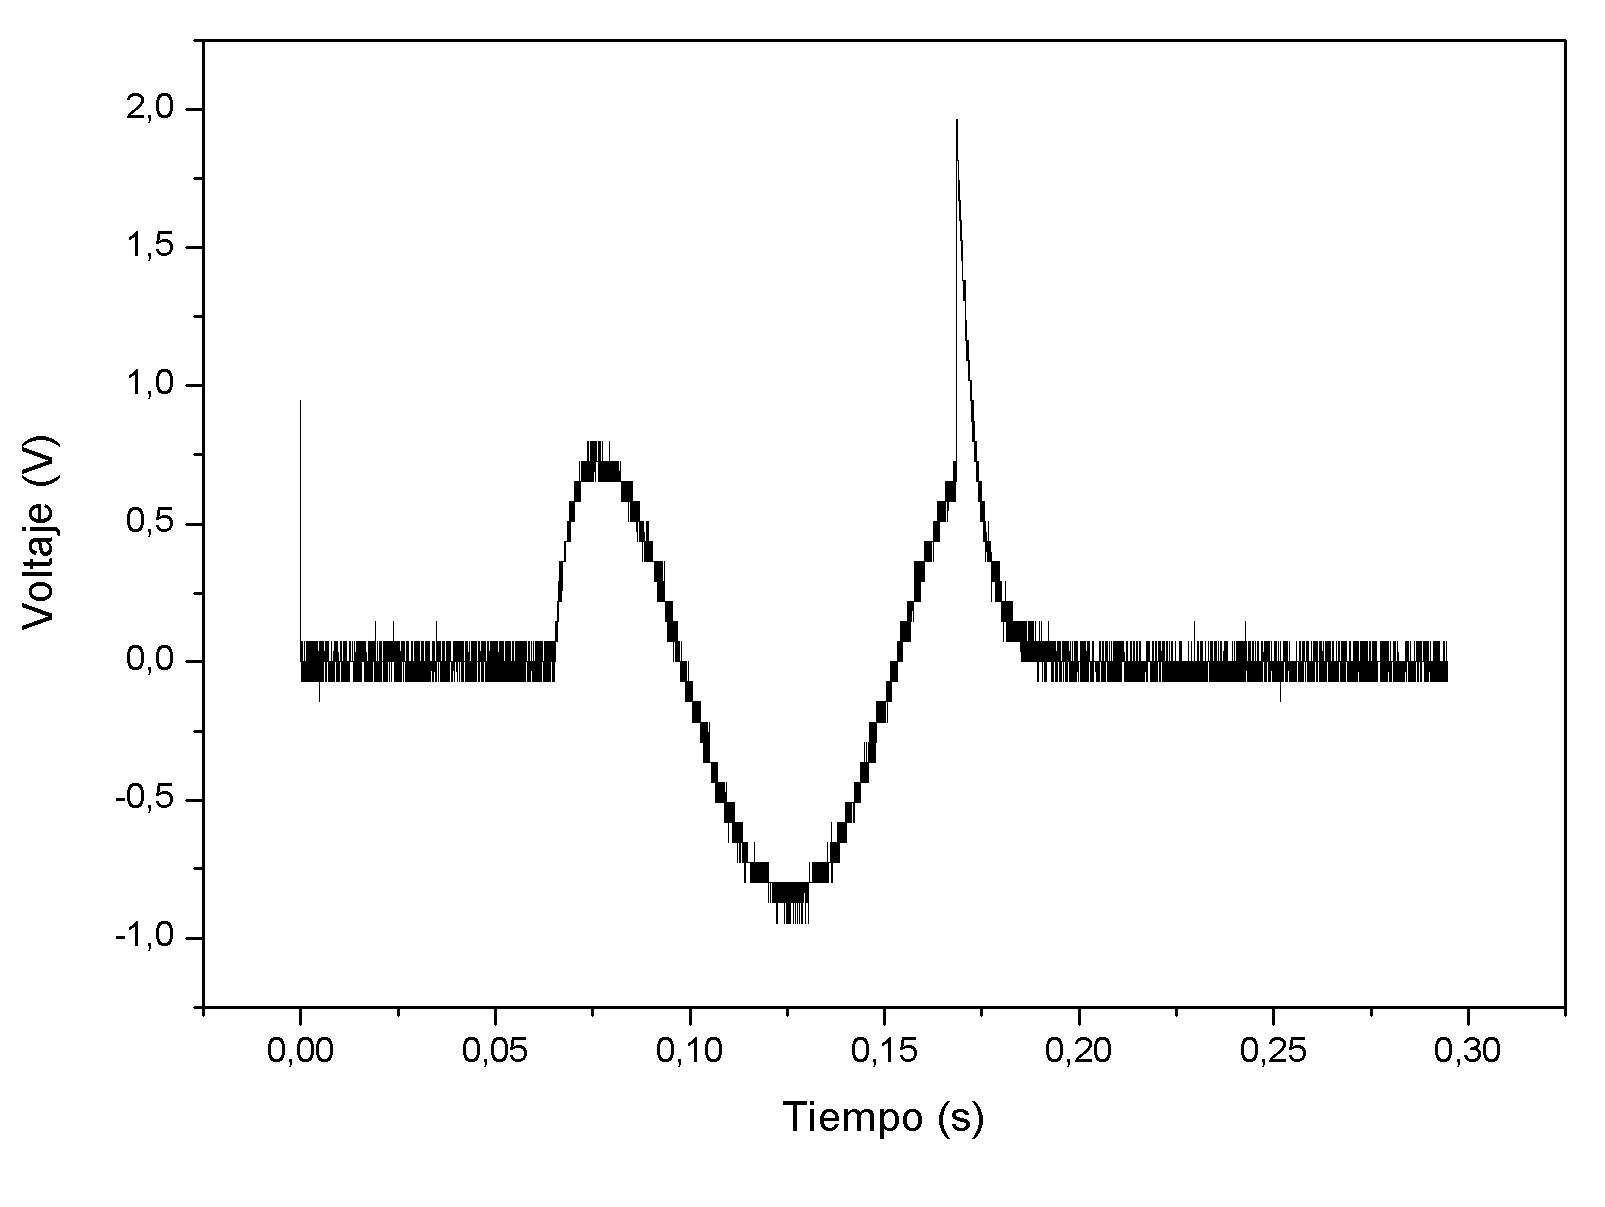
\includegraphics[width=0.40\textwidth]{V2-f1Hz.jpg} (a)
 \hspace{0.1cm}
 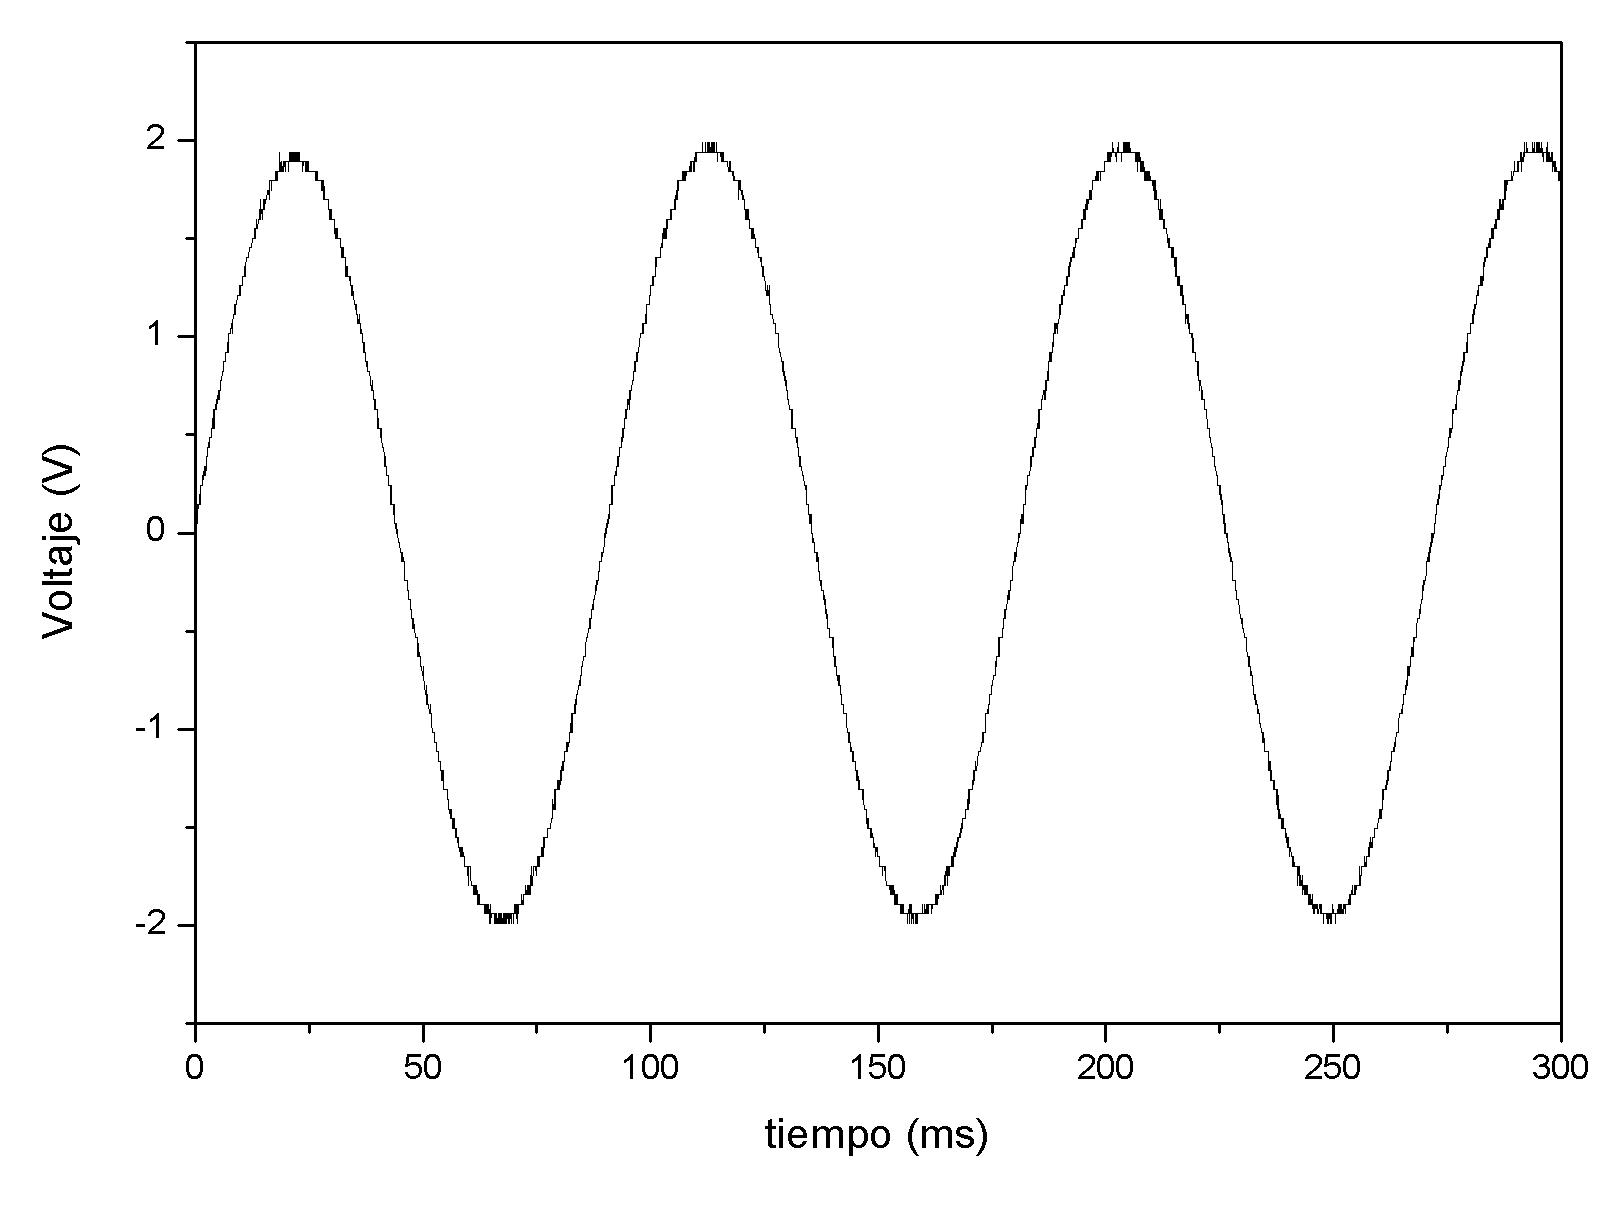
\includegraphics[width=0.40\textwidth]{V2-f10Hz.jpg} (b)  \\
 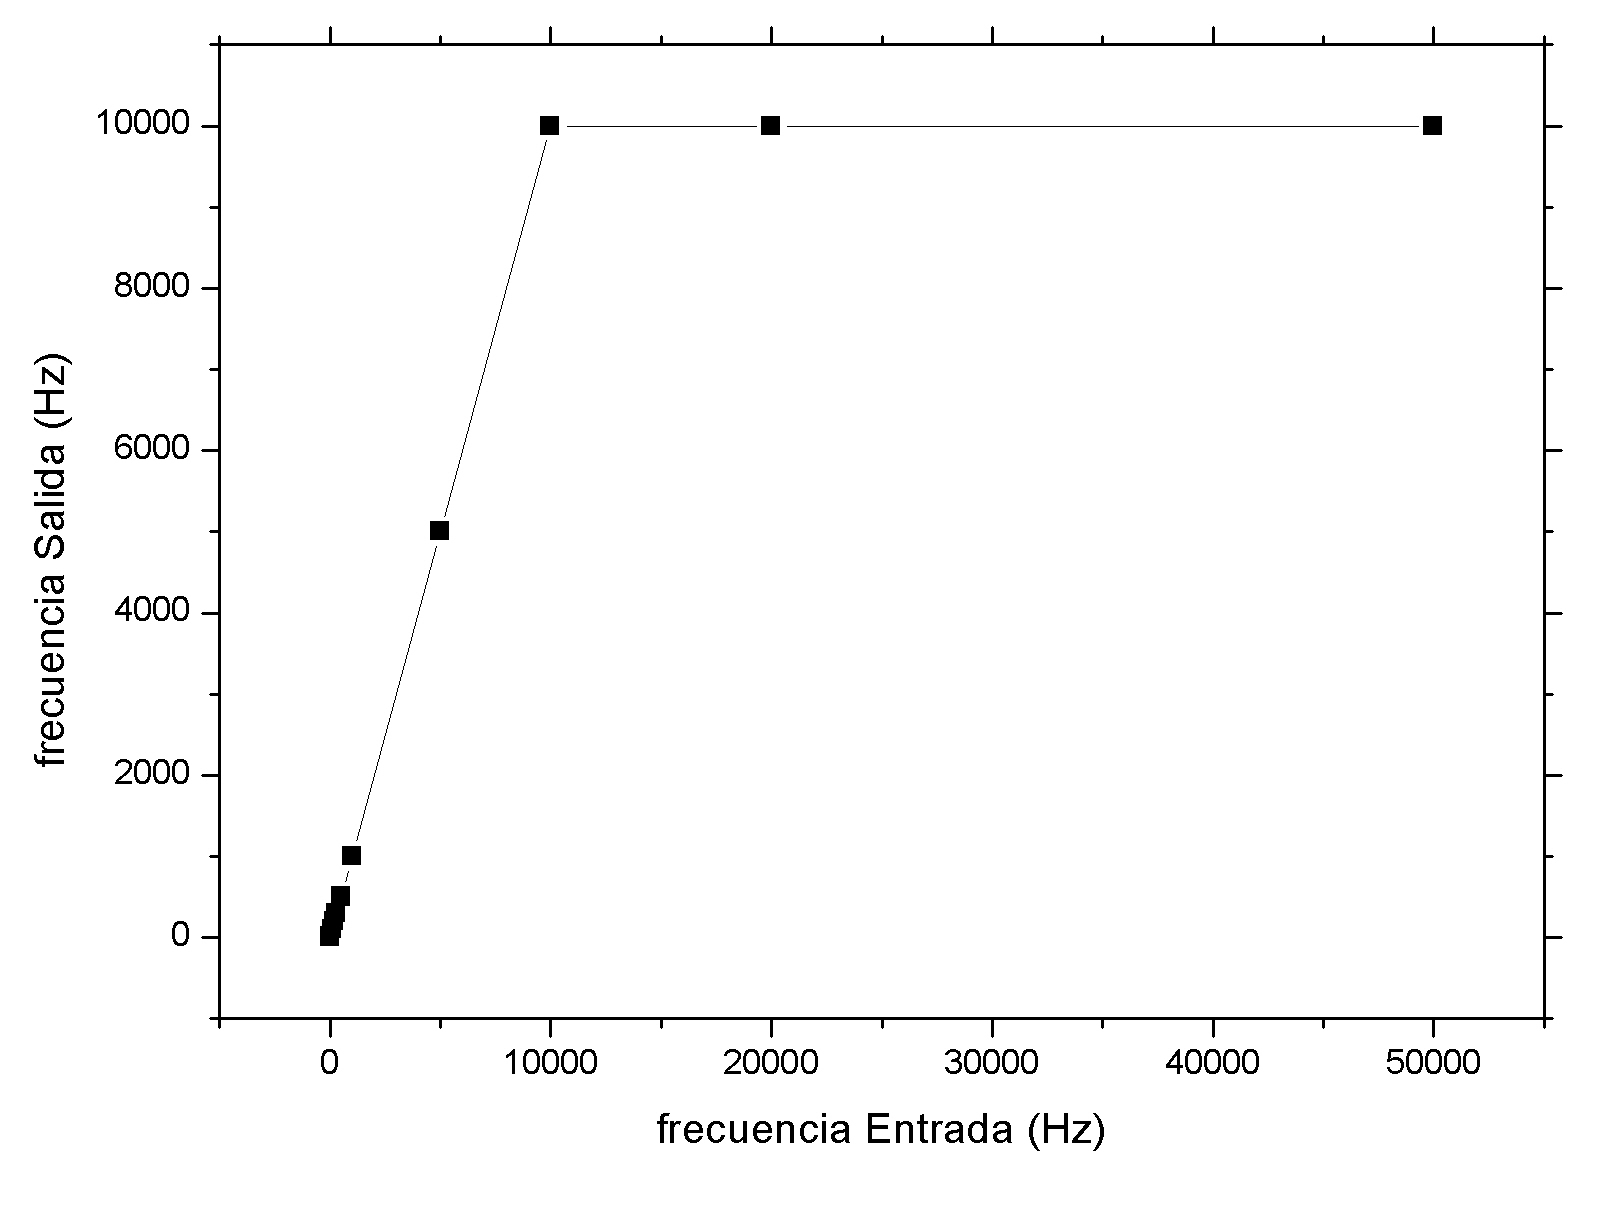
\includegraphics[width=0.40\textwidth]{FrecuenciaEntradaSalida.jpg} (c)
 \label{fig:frecuencia}
 \caption{Medidas de la señal de salida de una onda sinusoidal de la placa de audio para 1 Hz (a) y 10 Hz (b). (c) Gráfico de las frecuencia de Salida, respecto a la frecuencia de entrada.}
\end{figure}

%\subsection{Respuesta en voltaje de la placa de audio}
\vspace{0.5cm} \noindent
\textbf{\large 1.3 Respuesta en voltaje de la placa de audio} \vspace{0.25cm}

Para analizar los valores de voltaje que pueden aplicarse con la placa de audio se utilizaron variables del tipo Float32, con valores entre 1 y $-1$. A partir de valores mayores a $\pm1$, la señal saturaba, lo que resultaba en una deformación de la señal de salida. Esto se puede ver claramente en los resultados presentados en la Figura 2.

\begin{figure}[h!]
 \centering
 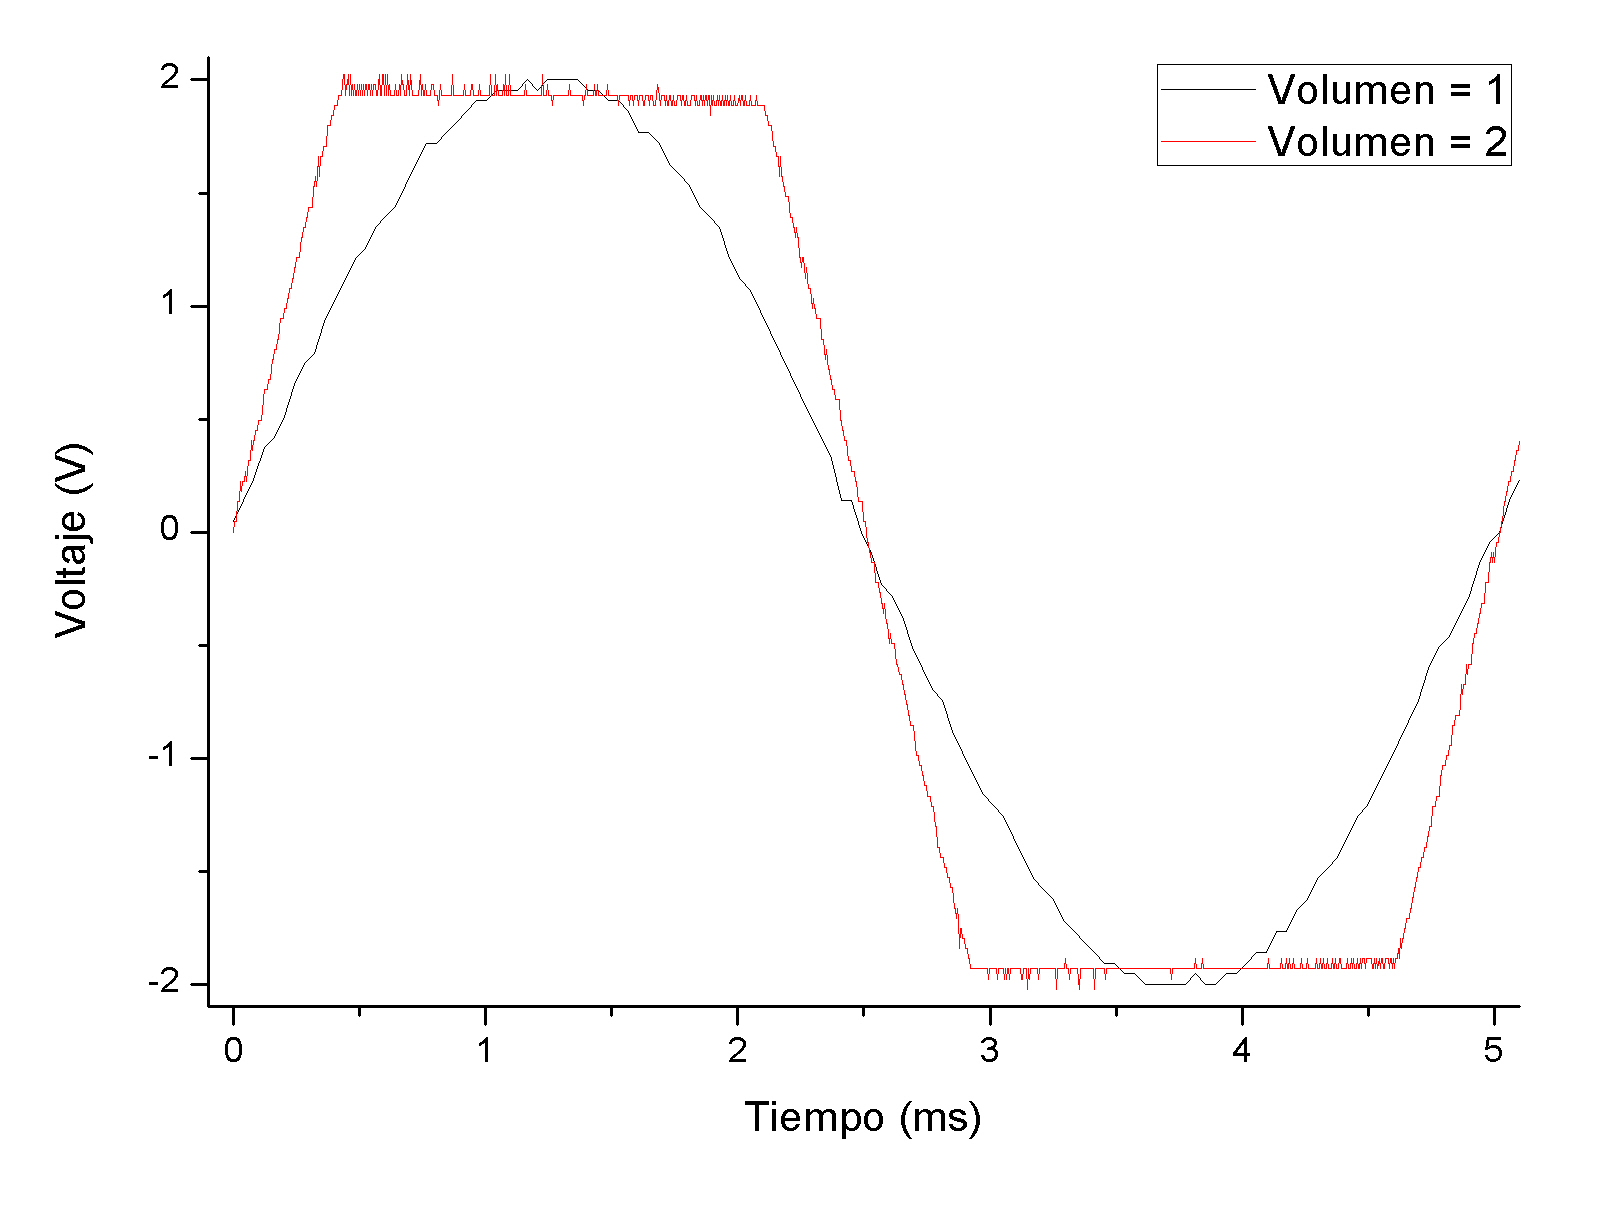
\includegraphics[width=0.40\textwidth]{Entrada-Volumen.jpg} (a)
 \hspace{0.1cm}
 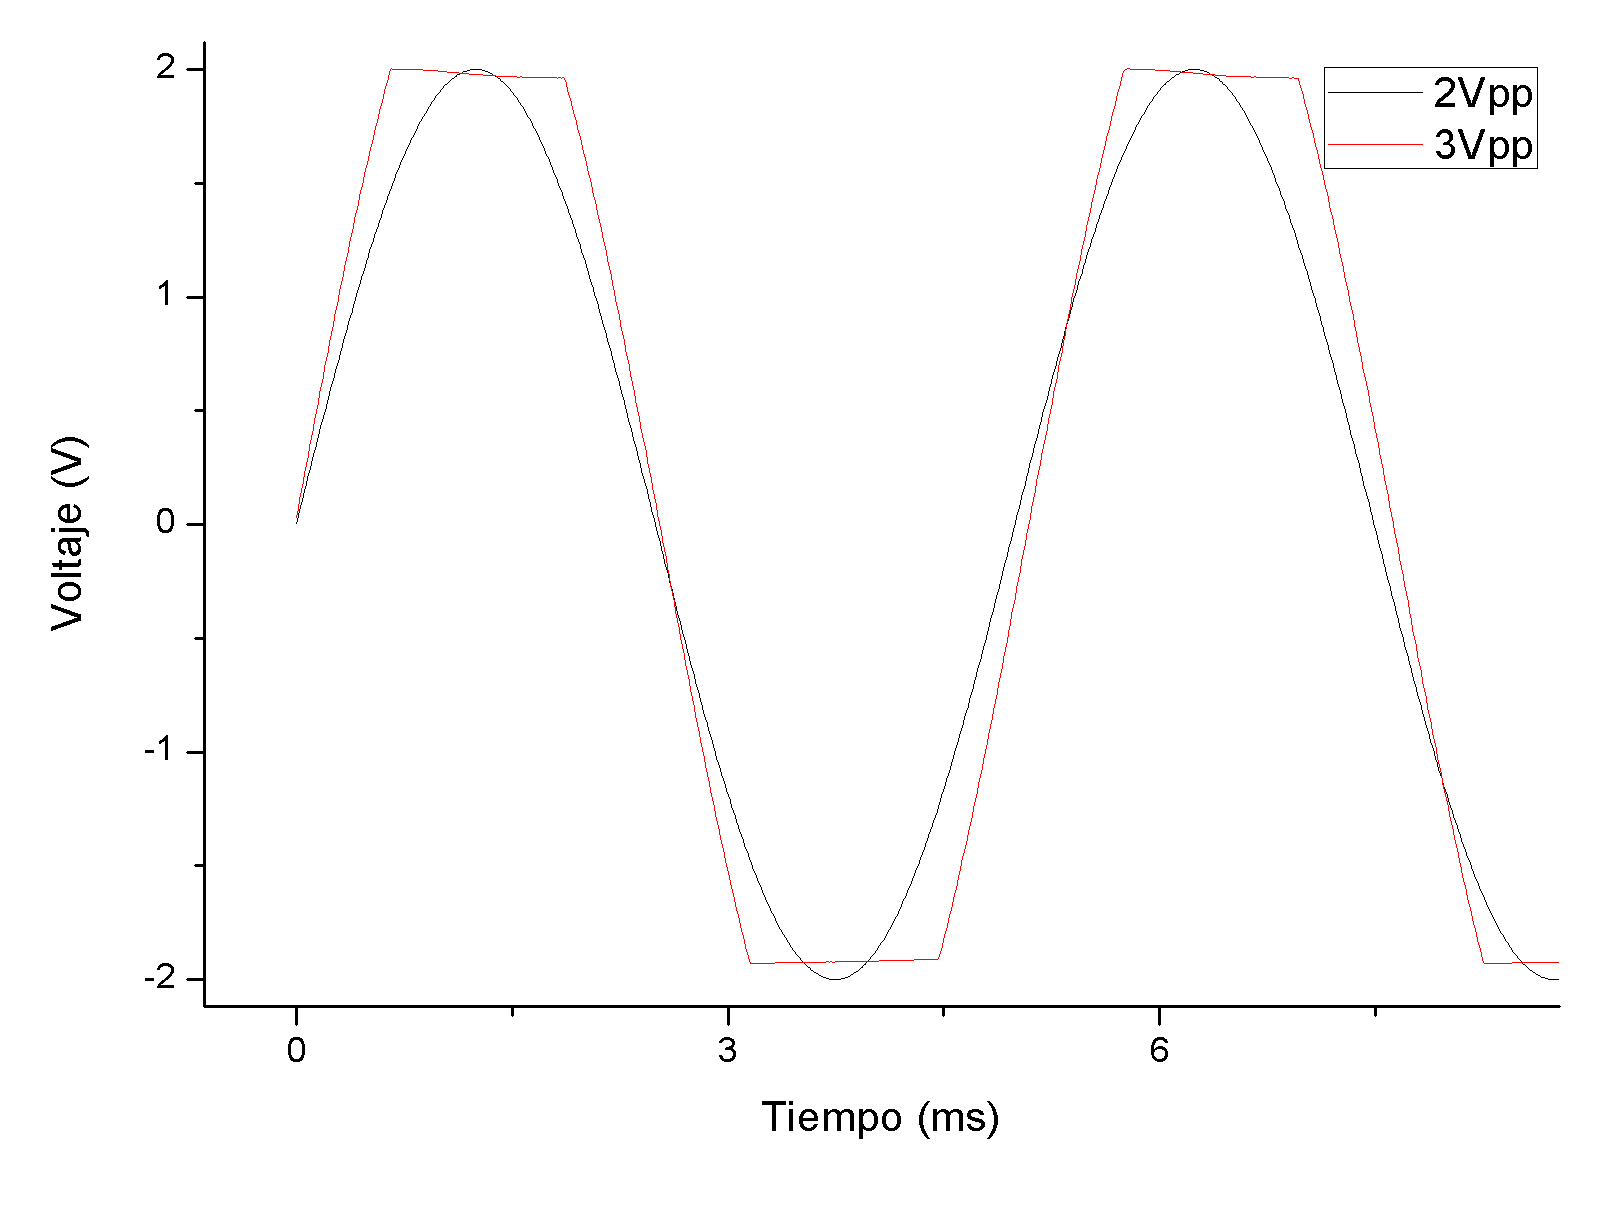
\includegraphics[width=0.40\textwidth]{PlacaAudio-Adq.jpg} (b)
 \label{fig:voltaje}
 \caption{Medidas de la señal de salida de la placa de Audio para ondas sinusoidales con frecuencia de 200 Hz y con el volumen máximo $V=1$ (a) e intentando sobrepasarlo $V=2$ (b).}
\end{figure}

Un resumen de la caracterización de entrada y salida de la placa de audio utilizada puede encontrarse en la Tabla~\ref{tab:inout-audio}.
\begin{table}[h]
\begin{tabularx}{\textwidth}{b|s|s|s }
Característica & Min & Máx & Unidad \\
\hline
Voltaje señal de entrada & 2 & -2 & V \\ 
Voltaje señal de salida & -2 & 2 & V \\
Frecuencia señal de entrada & 1 & 10000 & Hz \\
Frecuencia señal de salida & 10 & 10000 & Hz 
\end{tabularx}
\label{tab:inout-audio}
\caption{Caracterización de señales de entrada y salida de la placa de audio.}
\end{table}

\section{Determinación de curva de respuesta de diodo}
\label{sec:diodo}

Para probar las capacidades básicas de la placa de audio como generador de ondas, se medió la curva de  voltaje--corriente de un diodo. Para esto, se implementó el circuito que se muestra en la Figura 3a. La curva I-V de respuesta del diodo se muestra en la Figura 3b. Puede verse que la caída del diodo es de aproximadamente 0.67 V, lo cual es esperable en este sistema. Para poder definir las tierras del circuito de manera correcta, las conexiones de la señal de salida recolectadas por el osciloscopio fueron definidas de forma invertida. De manera, que la señal recolectada fue posteriormente
multiplicada por $-1$. 
%Cabe destacar que a la curva obtenida se multiplicaron por -1, dado que por la forma en que se conectó el osciloscopio, para que no haya problemas de tierras, estos valores estaban invertidos. 
La señal de entrada generada por la placa de audio tenía 2~V de amplitud y una frecuencia de 200~Hz.


\begin{figure}[h!]
 \centering
 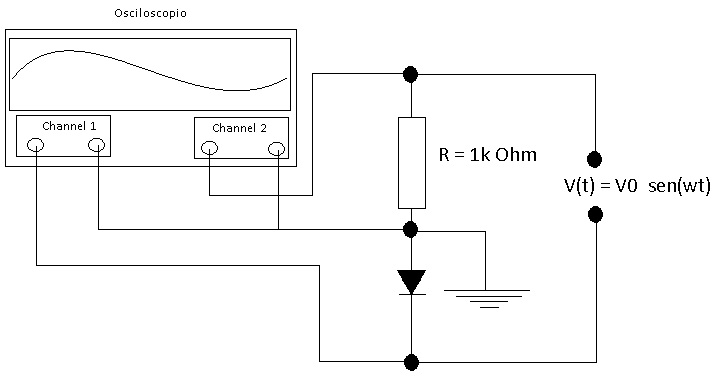
\includegraphics[width=0.5\textwidth]{circuit.jpg} (a)
 \hspace{0.1cm}
 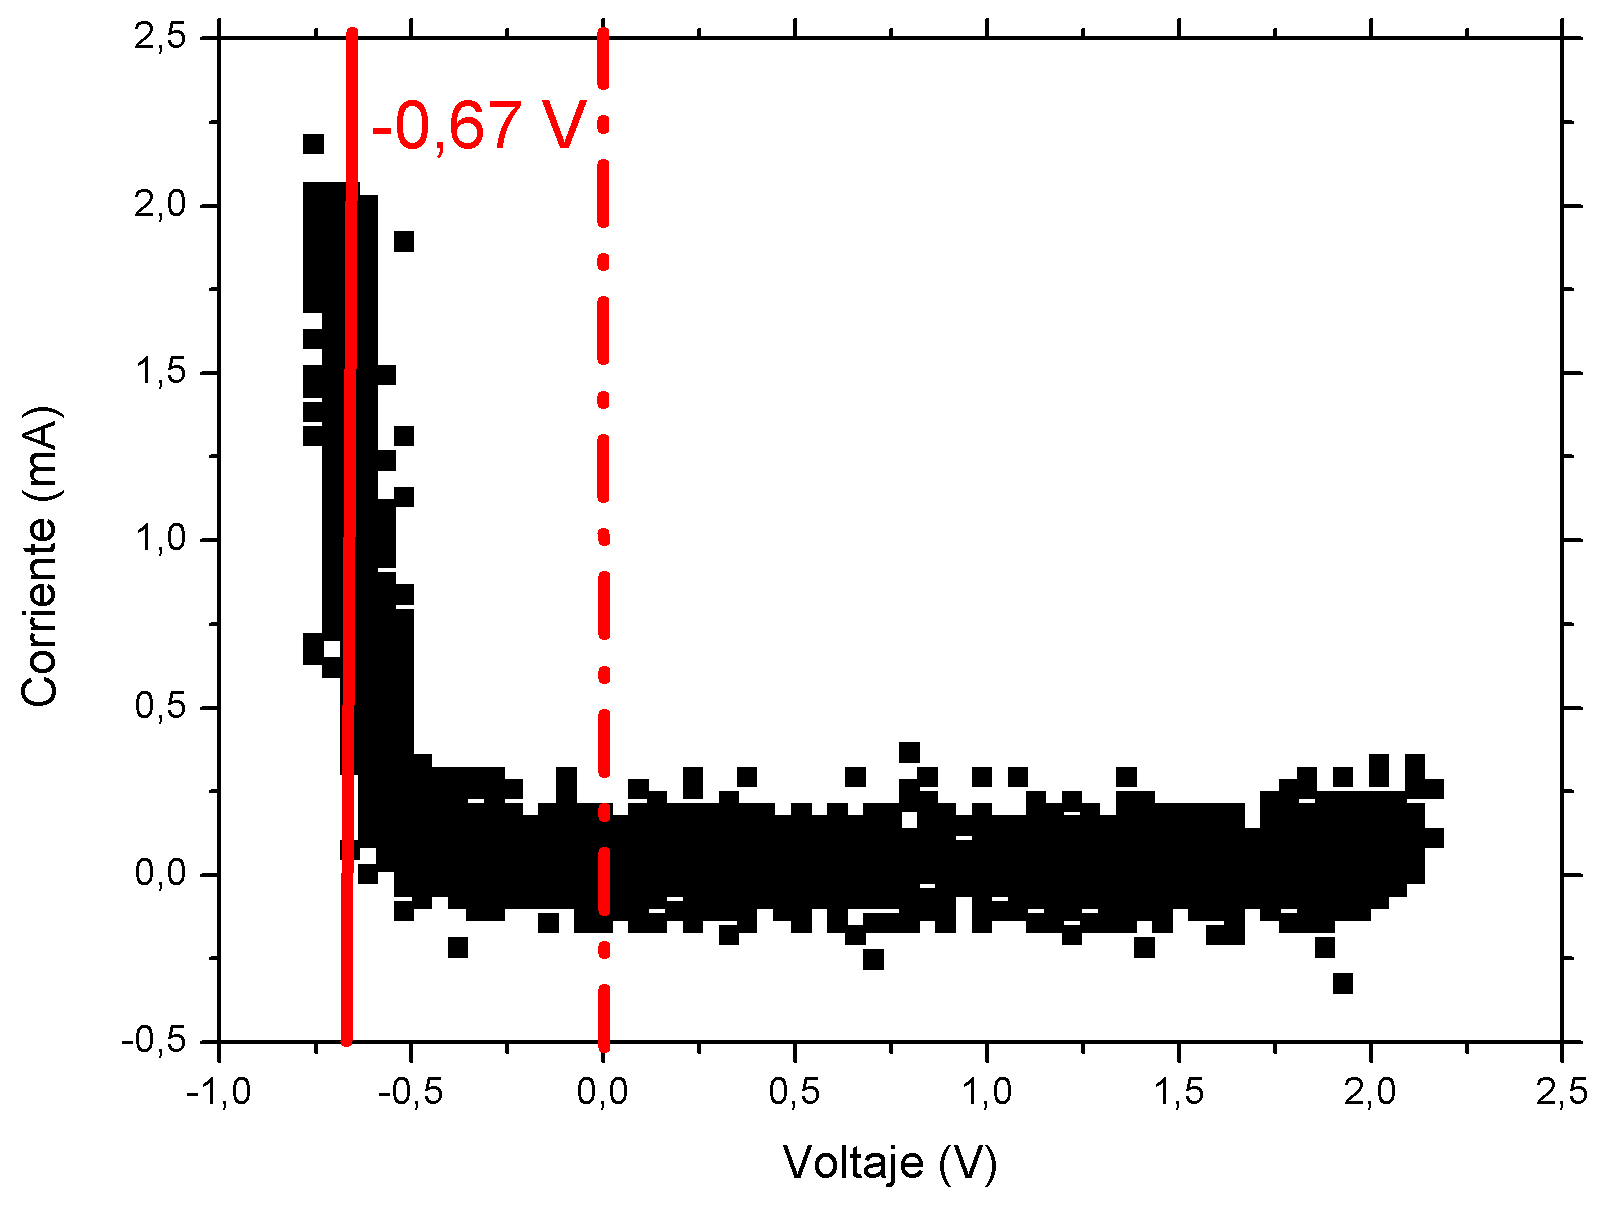
\includegraphics[width=0.35\textwidth]{DidoVoltajeCorriente2.jpg} (b)
 \label{fig:diodo}
 \caption{(a) Esquema del circuito implementado. 
 (b) Curva I-V del diodo.}
\end{figure}


\section{Implementación de OPAMP}
\label{sec:opamp}

Se pusieron en práctica dos diseños de circuito con amplificadores 
operacionales. El primero consistió en un amplificador inversor, y el segundo fue un circuito que permita determinar el {\it slew rate}. Los diagramas correspondientes se muestran en la Figura 4, en ambos casos se implementó
un LM741.

\begin{figure}[h]
 \centering
 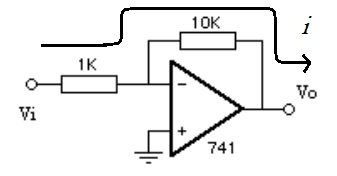
\includegraphics[width=0.4\textwidth]{AmpInv.png}(a)
 \hspace{0.1cm}
 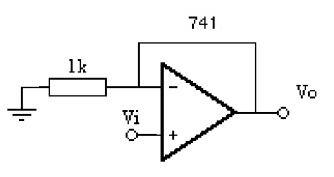
\includegraphics[width=0.4\textwidth]{slewratecircuit.png}
 (b)
 \label{fig:opamp}
 \caption{Diseño del circuitos: (a) Inversor amplificador y (b) para determinar el {\it slew rate}.}
\end{figure}

El circuito amplificador inversor se alimentó con una señal de 1 V de amplitud y 200 Hz generado por la placa de audio. Los resultados del amplificador inversor se muestran en la Figura 5-a. Puede verse que la señal sale invertida y multiplicada por un factor 10. 

No se pudo determinar el {\it slew rate} mediante la placa de audio, dada la limitación de ésta en frecuencia. Sin embargo, se presentan las medidas realizadas con un generador de onda y un osciloscopio en la Figura 5-b. Se utilizó un voltaje de 2~$V_{PP}$ y una frecuencia de 5 kHz de una onda cuadrada. A partir de los datos se calculó un {\it slew rate} de 0.507 $\pm$ 0.002 $\frac{V}{\mu s}$.

\begin{figure}[H]
 \centering
 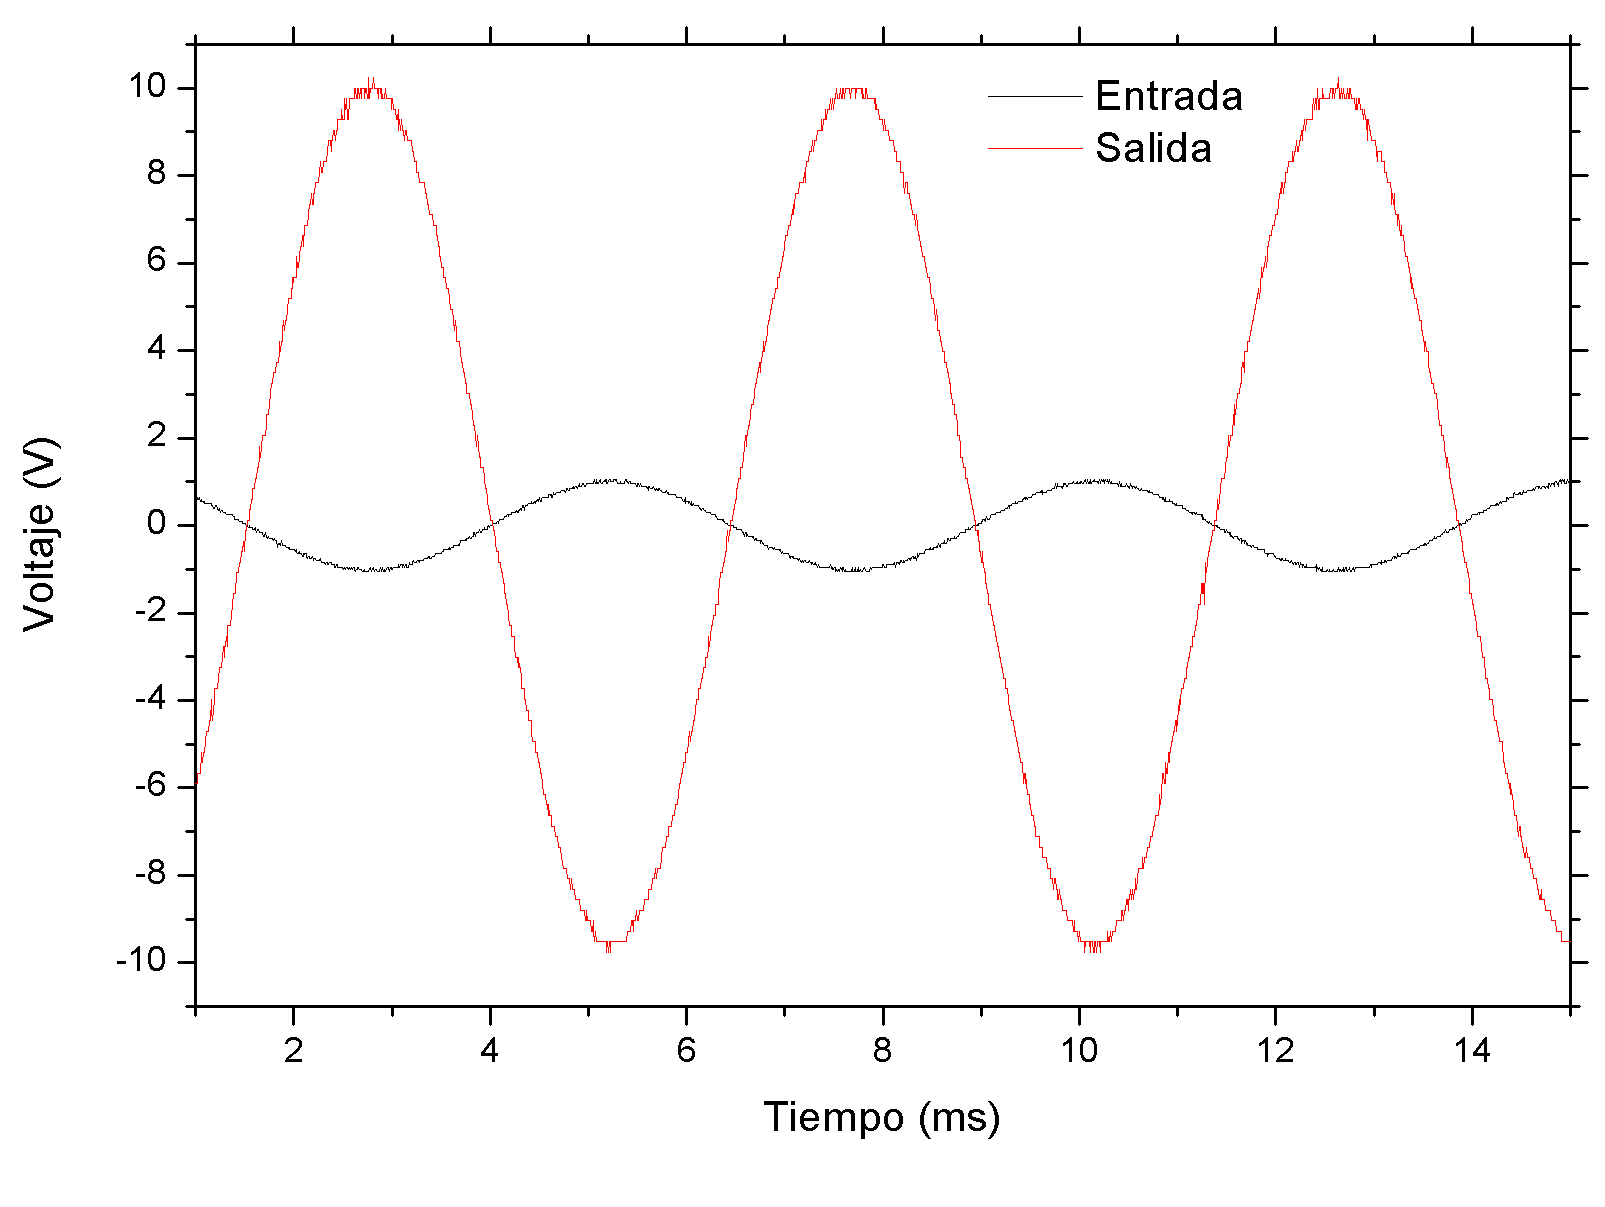
\includegraphics[width=0.45\textwidth]{AmplificadorInversor.jpg} 
 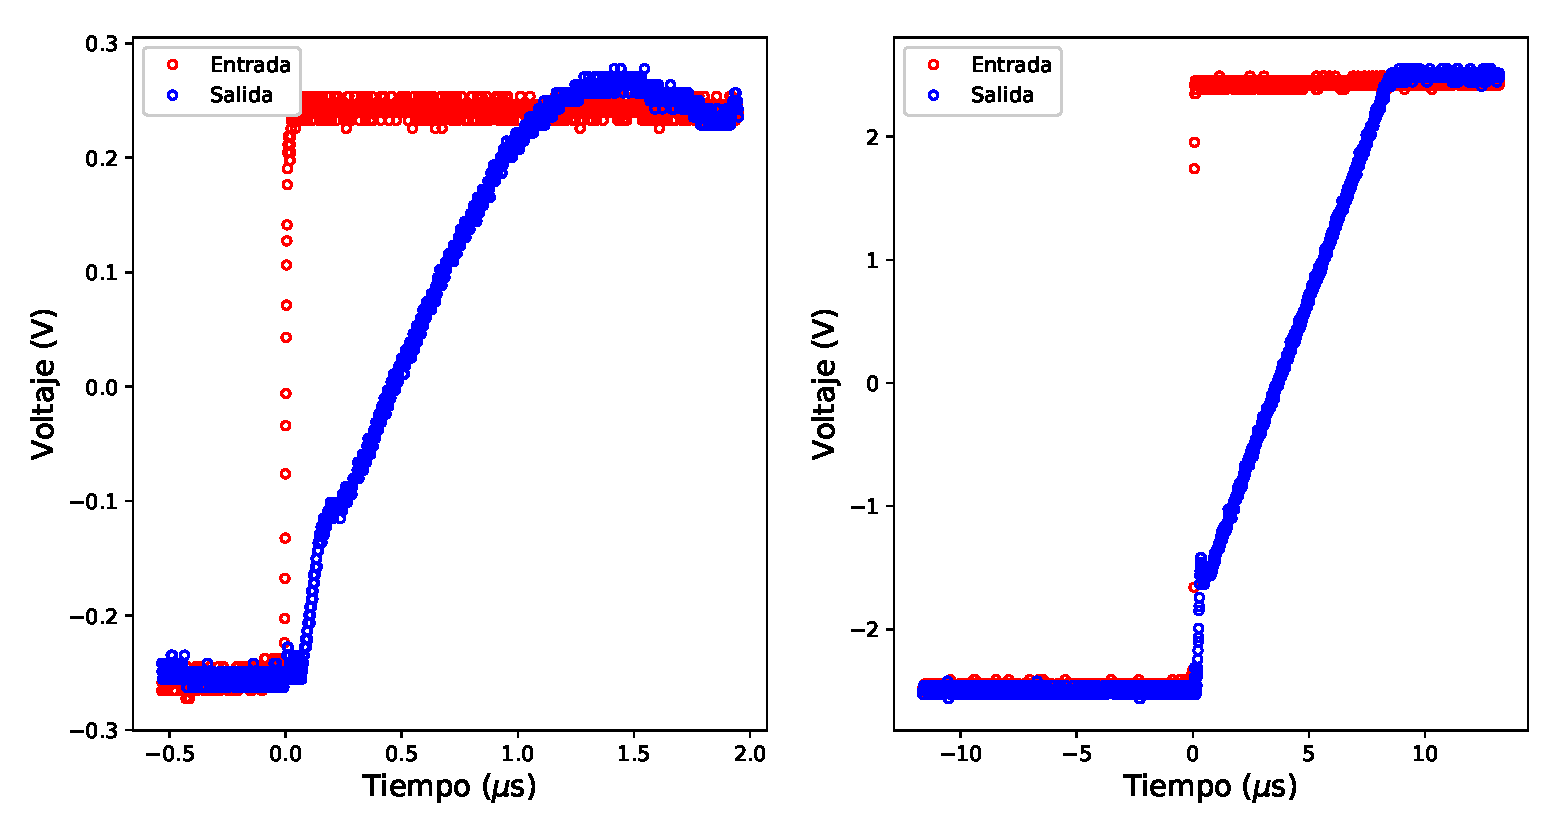
\includegraphics[trim={0 0 13cm 0},clip, width=0.32\textwidth]{slewrate.eps}
 \\
 \hspace{0.2cm}(a)\hspace{4.5cm}(b)
 \label{fig:slewrate}
 \caption{(a) Señales de entrada y salida del amplificador inversor, alimentado con una onda de 1 V de amplitud y 200 Hz de frecuencia. (b) Señales de entrada y salida de una onda cuadrada de
 2 V$_{PP}$ y 5kHz de frecuencia.}
\end{figure}

\end{document}
